\documentclass[11pt]{article}
\usepackage[sorting=none]{biblatex}
\usepackage{graphicx} 
\usepackage[font=scriptsize,labelfont=bf]{caption}
\usepackage[a4paper, total={5.5in, 8.5in}]{geometry}
\usepackage{cleveref}
\addbibresource{bibliography.bib}


\title{Xcorr Reimplementation Bachelorthesis}
\author{Michael zusmanovskiy}
\date{November 2024}

\begin{document}

\begin{titlepage}
    \begin{center}
        \LARGE
        Applied Computer Science

        \vspace{1cm}
        
        \LARGE
        Bachelorthesis

        \vspace{1cm}
            
        \LARGE
        \textbf{Re-implementation of the X-Corr algorithm in Python and improvement of scoring using predicted spectra}
            
        \vspace{1cm}

        \LARGE
        \textbf{Author}
        
        Michael Zusmanovskiy, 108019231182
        
        \vspace{1cm}
        
        \LARGE
        \textbf{Supervisors}
        
        Jun.-Prof. Julian Uszkoreit
        
        M.Sc. Dirk Winkelhardt
            
        \vfill
        
        \begin{figure}[ht]
            \centering
            \includegraphics[width=0.2\textwidth]{figs/Ruhr-Universität_Bochum_logo.svg.png}
        \end{figure}
            
        \Large
        Ruhr-Universität Bochum\\
        
        Submission date: 30. 12. 2024
            
    \end{center}
\end{titlepage}


\section{Introduction}
\subsection{Fundamentals}
Mass Spectrometry (MS) is a method for measuring the mass to charge ratios (m/z) of components in a  chemical substance sample and analysis of its molecules \cite{mass-specrometer}. MS has a variety of applications \cite{ms-applications} reaching from forensic analysis, where it is used to trace evidence , over environmental analysis, for example to keep track of pollution or test drinking water, to clinical purposes where MS is used for genomics research or diabetes research \cite{ms-diabetes}.
Before mass spectrometry can be performed, the sample has to be prepared meaning that it is turned into a state that is a valid input for the mass spectrometer. This is done by either converting it into a gas phase for Gas Chromatography or into a liquid phase for Liquid Chromatography. In Gas chromatography the molecular components are separated by vaporization and dilution of the sample on basis of attributes like weight, size, or boiling point. Liquid chromatography on the contrary separates components on basis of how fast they travel trough a liquid phase, this can be for example because of the difference of the polarity of the liquid phase and the components of the sample. Of course, the exact workflow is dependant on the Instrument that is used. Mass spectrometers exist in various variants e.G. MALDI-TOF MS, Triple Quadrupole MS, Hybrid Linear Ion Trap Orbitrap MS etc.  \cite{mass-specrometer-types} however regardless of their type they usually follow the same steps \cite{mass-specrometer, what-is-mass-spectrometry}: 

\begin{enumerate}
\item After the sample preparation, the sample is ionized, meaning that ions are generated. A common approach in gas chromatography is electron bombardement where the molecules are passed through a ionization chamber with accelerated electrons. The electrons collide with the molecules, break their bonds and turn them into fragments. A different approach in liquid
chromatography is electrospray chromatography where the liquidified sample is sprayed into an electric field where it evaporates.
\item The produced ions are sorted by their mass-to-charge ratios by a mass analyser. How this is done is dependant on the machine that is used.
\item After the sorting of the ions a detection system determines the relative abundances for each observed mass-to-charge (m/z) value.
\end{enumerate} 

The output is a mass spectrum which is a plot that yields the m/z values on the x-axis and the abundances on the y-axis. The m/z value is the mass of a particle divided by its electrical charge. The abundances are normalised to the highest abundance peak in the spectrum, meaning that the highest peak is 1 and all other peaks have a value relative to it, see \cref{fig:peptide-example}. 

Tandem mass spectrometry (MS/MS or \(MS^2\)) is used for the analysis of peptides and involves multiple stages, where in the first stage the entire sample is analysed with a mass spectrometer, then one ion is selected for further analysis and on the next stage only this isolated ion is analysed by another MS run \cite{tandem-mass-spectrometry}. 

Since every peptide sequence produces its own unique mass spectrum, it can be used as its unique fingerprint to identify it in a sample. 
\begin{figure}[ht]
    \centering
    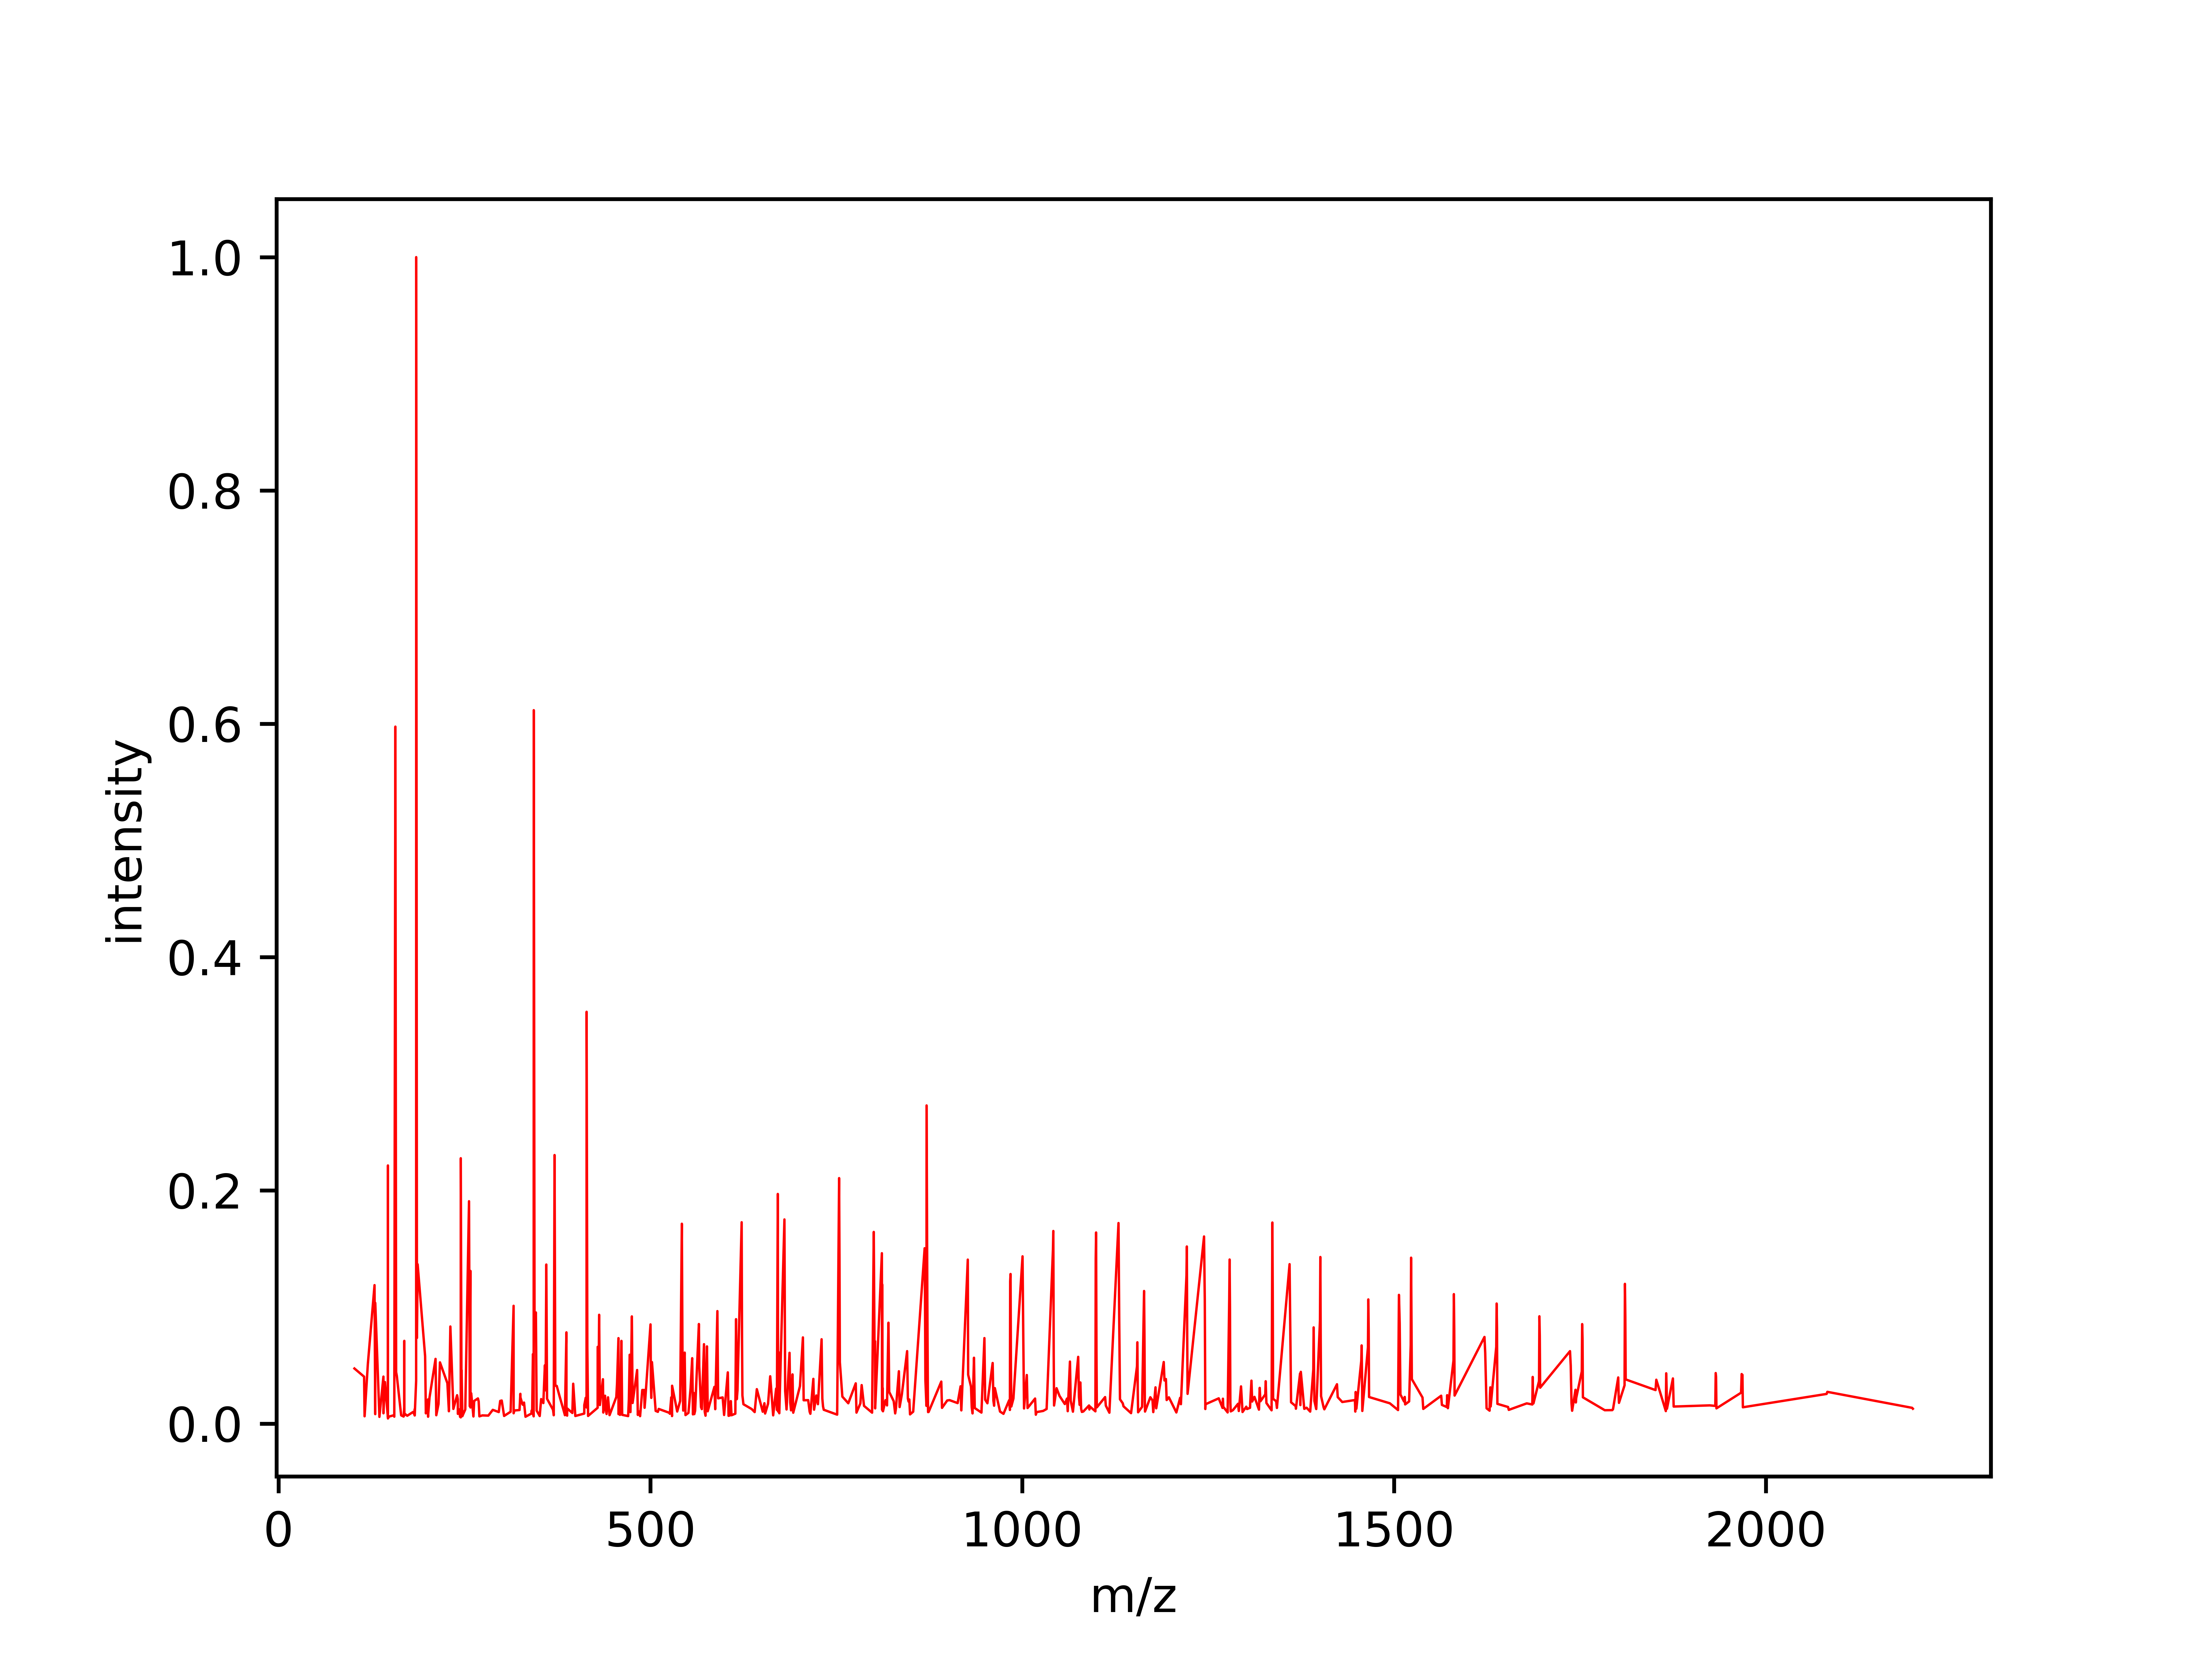
\includegraphics[width=0.8\textwidth]{figs/peptide.png}
    \caption{MS spectrum of the peptide "LAADEDDDDDDEEDDDEDDDDDDFDDEEAEEKAPVK" retireved from the human genome}
    \label{fig:peptide-example}
\end{figure}

Tandem MS searching is used for peptide identification within a mass spectrometry scan. Proteomics software that deals with the problem of identifying protein/peptide identification can fall into the category of database searching, where the search is performed against a database, and de novo searching, where peptides are deduced without a database.

\subsection{Motivation}
Comet is an open source proteomics Tandem MS/\(MS^2\) database search algorithm/tool written in C++ for searching spectrum data against sequence databases and identification of peptides, that in 2012 emerged from the SEQUEST database search tool from the University of Washington that was written in 1994 \cite{comet-search-tool}. It supports multithreading and is highly parametrizable. The tool computes multiple scores that evaluate how close a sample peptide is to the peptide it is compared to. One of these scores is the "xcorr". To calculate the xcorr value the algorithm constructs a spectrum from the peptide which is assumed to be the peptide of the sample by generating all possible m/z values from the 'b' and 'y' series of the peptide \cite{comet-first-paper}. Since in 1994 it was not entirely possible to predict the intensities of 'b' and 'y' ions, they are assigned the intensity of 1 \cite{deeper-look-into-comet}. Neighboring m/z values, meaning $\pm$1 m/z, receive an intensity of 0.5. With the sample spectrum and the constructed "theoretical" spectrum, a correlation based score is computed
to evaluate the fitting of the found peptide.

Peptide prediction algorithms are able to predict \(MS^2\) peaks with the help of various machine learning models.
MS2PIP\cite{ms2pip} is a command line peptide intensity prediction tool which also exposes a python API.

This work wants to combine the comet cross-correlation scoring algorithm
with the peptide intensity prediction of MS2PIP to create an even more accurate identification of peptides.


\subsection{Goals}
As comet is written in the C/C++ Programming Languages and MS2PIP is a Python Api, it is first of all necessary to translate the Comet cross-correlation scoring algorithm to the python programming language as accurately as possible. Next, the theoretical spectrum containing only m/z values without any abundances created by comet will be replaced by the predicted spectrum of MS2PIP. Performance regarding computational speed and identified peptides will be then compared to the initial comet algorithm, and the to python translated comet.
The goal of this work is to check whether replacing comets theoretical spectrum with the predicted spectrum of MS2PIP will yield better results in peptide identification, and with this, to find a new method of peptide identification.

\section{Methods and Structure}
\subsection{Realizing the Xcorr algorithm in Python}
For this work, Python is used as the Programming language. Before implementing, it is first necessary to have human genome data to work with. For this purpose, LFQ Orbitrap data was used as the sample, specifically in the mzml format which is a xml based format for storing mass spec scan data. The search is done against data of the human genome in the fasta format which stores protein primary structure and serves as the "database".

\subsubsection{Reading in Spectrum data}
Acessing these files with python was done with the help of the pyteomics framework \cite{pyteomics, pyteomics-five-years} which contains many tools for working with proteomics data. For efficient identification of peptides it is first necessary to create a compact list that contains all masses, and peptides that have this mass.

\subsubsection{CLI}
To make usage comfortable, a CLI is implemented. This was done with the help of the Typer library. The general usage is "cli.py [OPTIONS] SAMPLE\_FILENAME PROTEIN\_DATABASE" in the terminal, where "SAMPLE\_FILENAME" is a required argument and placeholder for the sample filename in the mzml format as a string, and "PROTEIN\_DATABASE" the string for the database filename of the human genome respectively.






\section{Discussion and Conclusion}
\subsection{Evaluation}
\subsection{Future Work}
\subsection{Impact \& Conclusion}


\printbibliography

\end{document}
